% !TEX encoding = UTF-8
% !TEX TS-program = pdflatex
% !TEX root = ../tesi.tex

%**************************************************************
\chapter{Introduzione}
\label{cap:introduzione}
%**************************************************************

Questa tesi descrive l'esperienza e il percorso lavorativo svolto presso l'azienda Gruppo4 sotto la supervisione di Tobia Conforto.

%**************************************************************
\section{L'azienda}
Gruppo4 è una web agency Padovana, da oltre vent'anni ha accumulato competenze e l'esperienza necessaria per fornire soluzioni efficaci e innovative nel settore web. Mediante un modello organizzativo consolidato e certificato sviluppano applicazioni web che si distinguono per la chiarezza dell'interfaccia utente (UX/UI) e per la loro usabilità.

%**************************************************************
\section{Gli obiettivi del progetto}
L'obiettivo principale di questo progetto consiste nella realizzazione di un componente di interfaccia grafica per il web in Kotlin. Il componente deve essere una tabella pivot interattiva che permette ad un utente la possibilità di esplorare liberamente i \emph{big data} contenuti al suo interno. Oltre alla realizzazione del componente, questo progetto ha anche lo scopo di valutare l'efficacia di Kotlin nel realizzare interfacce utente per il web in quanto l'azienda utilizza già Kotlin nello sviluppo di \gls{api}.

%**************************************************************
\section{Tabella pivot}
L'azienda mi ha fornito una descrizione accurata della tabella pivot per quanto riguarda la sua struttura e le sue funzionalità. Nelle prossime sottosezioni descriverò gli elementi che la compongono e le possibili interazioni con l'utente. \\
Durante la discussione dei requisiti del componente, l'azienda mi ha fornito un accesso ad una istanza della loro applicazione correntemente in uso. Mi sono stati forniti dei dati da usare nello sviluppo del componente ed un accesso all'interfaccia di una tabella esistente per capire al meglio il suo funzionamento. \\
\begin{minipage}{\linewidth}
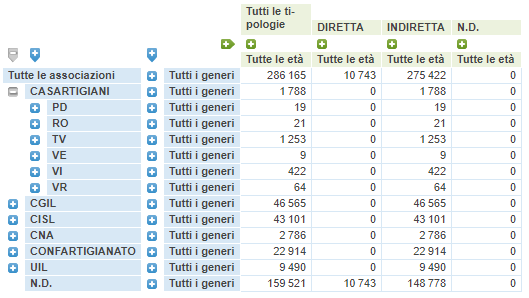
\includegraphics[scale=0.75]{./immagini/tabella-pivot-old.png}
\captionof{figure}{Screenshot tabella realizzata da Gruppo4}
\end{minipage}

\subsection{Struttura}
La tabella pivot si può suddividere in tre parti ben distinte: le celle contenente i dati, le celle d'intestazione delle righe e quelle delle colonne. 
Le celle d'intestazione sono definite come le \emph{dimensioni di analisi} della tabella. Esse rappresentano tutte le variabili riguardanti i dati contenuti nella tabella. Le \emph{dimensioni di analisi} della tabella pivot possono essere molteplici sia per le righe che per le colonne. Ad esempio, nello screenshot precedente, le \emph{dimensioni di analisi} delle righe sono l'insieme delle due variabili: Associazioni e Genere. Quindi ogni cella dei dati corrisponde ad una intersezione tra le \emph{dimensioni di analisi} delle righe e delle colonne.

\subsection{Funzionalità}
La tabella deve essere completamente esplorabile da un utente, per farlo bisogna identificare le azioni che possono essere eseguite:
\begin{itemize}
	\item aprire e chiudere tutti i figli di una dimensione;
	\item aprire e chiudere un singolo figlio di una dimensione.
\end{itemize}
Mediante queste azioni i big data possono essere esplorati ed analizzati dall'utente.

%**************************************************************
\section{Organizzazione del testo}
Riguardo la stesura di questo documento sono state adottate le seguenti convenzioni tipografiche:
\begin{itemize}
	\item gli acronimi, le abbreviazioni e i termini ambigui o di uso non comune menzionati vengono definiti nel glossario, situato alla fine del presente documento;
	\item la prima occorrenza dei termini riportati nel glossario viene indicata mediante una scrittua in blu;
	\item i termini in lingua straniera o facenti parti del gergo tecnico sono evidenziati con il carattere \emph{corsivo}.
\end{itemize}